\documentclass[letterpaper,12pt]{article}
\usepackage{array}
\usepackage{threeparttable}
\usepackage{geometry}

\usepackage{natbib}

%\usepackage{jf} %always check the instruction of the package to see if it conflicts
\geometry{letterpaper,tmargin=1in,bmargin=1in,lmargin=1.25in,rmargin=1.25in}
\usepackage{fancyhdr,lastpage}
\pagestyle{fancy}
\lhead{}
\chead{}
\rhead{}
\lfoot{}
\cfoot{}
\rfoot{\footnotesize\textsl{Page \thepage\ of \pageref{LastPage}}}
\renewcommand\headrulewidth{0pt}
\renewcommand\footrulewidth{0pt}
\usepackage[format=hang,font=normalsize,labelfont=bf]{caption}
\usepackage{listings}
\lstset{frame=single,
  language=Python,
  showstringspaces=false,
  columns=flexible,
  basicstyle={\small\ttfamily},
  numbers=none,
  breaklines=true,
  breakatwhitespace=true
  tabsize=3
}
\usepackage{amsmath}
\usepackage{amssymb}
\usepackage{amsthm}
%\usepackage{harvard}
\usepackage{setspace}
\usepackage{float,color}
\usepackage[pdftex]{graphicx}
\usepackage{hyperref}
\hypersetup{colorlinks,linkcolor=red,urlcolor=blue,citecolor=blue}
\theoremstyle{definition}
\newtheorem{theorem}{Theorem}
\newtheorem{acknowledgement}[theorem]{Acknowledgement}
\newtheorem{algorithm}[theorem]{Algorithm}
\newtheorem{axiom}[theorem]{Axiom}
\newtheorem{case}[theorem]{Case}
\newtheorem{claim}[theorem]{Claim}
\newtheorem{conclusion}[theorem]{Conclusion}
\newtheorem{condition}[theorem]{Condition}
\newtheorem{conjecture}[theorem]{Conjecture}
\newtheorem{corollary}[theorem]{Corollary}
\newtheorem{criterion}[theorem]{Criterion}
\newtheorem{definition}[theorem]{Definition}
\newtheorem{derivation}{Derivation} % Number derivations on their own
\newtheorem{example}[theorem]{Example}
\newtheorem{exercise}[theorem]{Exercise}
\newtheorem{lemma}[theorem]{Lemma}
\newtheorem{notation}[theorem]{Notation}
\newtheorem{problem}[theorem]{Problem}
\newtheorem{proposition}{Proposition} % Number propositions on their own
\newtheorem{remark}[theorem]{Remark}
\newtheorem{solution}[theorem]{Solution}
\newtheorem{summary}[theorem]{Summary}
%\numberwithin{equation}{section}
%\bibliographystyle{aer}
\newcommand\ve{\varepsilon}
\newcommand\boldline{\arrayrulewidth{1pt}\hline}

\DeclareMathOperator*{\argmax}{arg\,max}

\usepackage{graphicx}
\graphicspath{ {C:/Users/yafei/CompEcon_Fall17/ProblemSets/ProblemSet7} }

\title{Problem Set 7: Web Scraping}
\author{Yafei Zhang \thanks{Yafei Zhang is from Finance department of USC, he can be reached at yafei.zhang@grad.moore.sc.edu.}}
\date{November 13, 2017}

\begin{document}

\maketitle

\vspace{5mm}

\section{Introduction}

In this problem set, I will investigate the long-run time-series trend of personal income in United States. The reason for me to analyze the time-series variation of personal income is that I want to have a sense of how banking deregulation affects the personal income. I collect state-level personal income per capita (PIPC, in dollars) from Bureau of Economic Analysis (BEA) from 1929 to 2016. The original dataset includes 5,280 state-year observations.

I first plot the national-level PIPC against years to gain a brief sense about the time-series variation of personal income. Then according to the definition of BEA, I split the sample into Great Lakes, Plains, Rocky Mountain, New England, Mideast, Southeast, Southwest, and Far West and compare them with each other\footnote{Please see https://www.bea.gov/regional/docs/regions.cfm for detailed information regarding these categories.}. This tells me the geographical variation of PIPC. Lastly, I single out California and study whether the PIPC has different pattern before the banking deregulation and after.

I find that U.S. personal income has experienced an exponential growth since 1929. Also, different regions show different time-series patterns, especially after 1980. Before 1980, personal income per capita is close to each other for different regions. While after 1980, they start to diverge. States included in New England grow fastest from 1980 to 2016, whereas states in south area (Southeast and Southwest) have the slowest growth. Then, in the case study of California, I find that the slope of the PIPC curve after intra-state banking deregulation is different from the slop of the curve before. Inter-state banking deregulation, however, seems to have no impacts on personal income in California. It is too early to say that intra-state banking deregulation affects the personal income growth rate, further analyses are needed.


\section{Relationships interpretation}

\subsection{Figure 1}

In this subsection, I plot time-series variation of national personal income per capita. Figure \ref{fig:figure1} shows the relationship. Y axis denotes the national level PIPC in dollars, x axis denotes the years. The figure covers data from 1929 to 2016. The relationship in the figure shows that PIPC increases exponentially. It reaches 50,000 dollars at 2016. Also, the slope of the curve changes around 1970s. It is worthwhile noting that most of the states passed banking deregulation legislation around 1970s.


\begin{figure}[h]
	\centering
	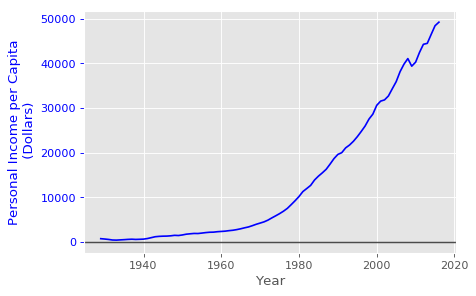
\includegraphics[width=\textwidth]{figure1}
	\caption{National Personal Income across Years}
	\label{fig:figure1}
\end{figure}



\subsection{Figure 2}

This subsection shows the results of Figure \ref{fig:figure2}. It plots the personal income per capita for different regions across years. 

A couple of facts surface from the picture. First, the slope changes around 1975. Second, before 1980, there is not much variation across different areas. But after 1980, personal income diverged. New England, Mideast, and Far West grow faster than the rest regions. Third, almost starting from 2000, the variations of personal income for each regions increased.

\begin{figure}[h]
	\centering
	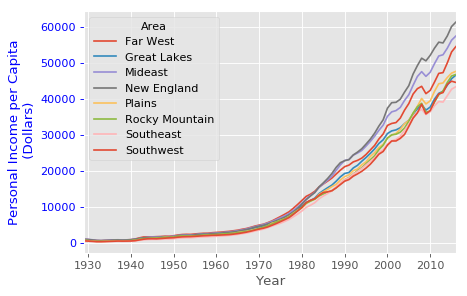
\includegraphics[width=\textwidth]{figure2}
	\caption{Regional Personal Income across Years}
	\label{fig:figure2}
\end{figure}


\subsection{Figure 3}

This subsection singles out California to visualize the potential impact of banking deregulation on personal income per capita.

The red line in the picture shows the time-series trend of personal income per capita for California. Similarly, the slope changed around 1970, the year when California passed the intra-bank deregulation legislation. The black dotted line denotes the year. The dotted line with blue color denotes year 1987 when the inter-state banking deregulation legislation was passed. As you can see, there was no significant pattern change of the personal income.

\begin{figure}[h]
	\centering
	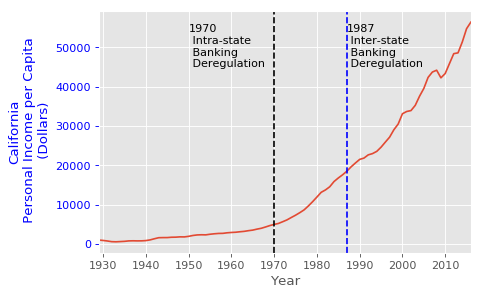
\includegraphics[width=\textwidth]{figure3}
	\caption{California Personal Income across Years}
	\label{fig:figure3}
\end{figure}




\end{document}